% How to use writeLaTeX: 
%
% You edit the source code here on the left, and the preview on the
% right shows you the result within a few seconds.
%
% Bookmark this page and share the URL with your co-authors. They can
% edit at the same time!
%
% You can upload figures, bibliographies, custom classes and
% styles using the files menu.
%
% If you're new to LaTeX, the wikibook is a great place to start:
% http://en.wikibooks.org/wiki/LaTeX
%
%%%%%%%%%%%%%%%%%%%%%%%%%%%%%%%%%%%%%%%%%%%%%%%%%%%%%%%%%%%%%%%%%%%%%%
% Edit the title below to update the display in My Documents
%\title{Project Report}
%
%%% Preamble
\documentclass[paper=a4, fontsize=11pt]{scrartcl}
\usepackage[T1]{fontenc}
\usepackage{fourier}

\usepackage[english]{babel}     % English language/hyphenation
\usepackage[protrusion=true,expansion=true]{microtype}	
\usepackage{verbatim}
\usepackage{amsmath,amsfonts,amsthm} % Math packages
\usepackage[pdftex]{graphicx}
\graphicspath{ {images/} }
\usepackage{caption}
\usepackage{subcaption}
\usepackage{url}
\usepackage{babel}
\usepackage{biblatex}
\addbibresource{reference.bib}
\usepackage{hyperref}

%%% Custom margins
\usepackage[hscale=0.75,vscale=0.75,vmarginratio={4:5},heightrounded]{geometry}

%%% Custom sectioning
\usepackage{sectsty}
\allsectionsfont{\centering \normalfont\scshape}

%%% Custom headers/footers (fancyhdr package)
\usepackage{fancyhdr}
\pagestyle{fancy}
\fancyhead{}											% No page header
\fancyfoot[L]{}											% Empty 
\fancyfoot[C]{}											% Empty
\fancyfoot[R]{\thepage}									% Pagenumbering
\renewcommand{\headrulewidth}{0pt}			% Remove header underlines
\renewcommand{\footrulewidth}{0pt}				% Remove footer underlines
\setlength{\headheight}{13.6pt}


%%% Equation and float numbering
\numberwithin{equation}{section}		% Equationnumbering: section.eq#
\numberwithin{figure}{section}			% Figurenumbering: section.fig#
\numberwithin{table}{section}				% Tablenumbering: section.tab#
\setlength{\parskip}{5pt}

%%% Maketitle metadata
\newcommand{\horrule}[1]{\rule{\linewidth}{#1}} 	% Horizontal rule

\title{
		\vspace{-1cm}
		\usefont{OT1}{bch}{b}{n}
		\normalfont \normalsize \textsc{CSCI 580, Prof. Saty Raghavachary} \\ [25pt]
		\horrule{0.4pt} \\[0.5cm]
		\huge\textbf{Crepescular Rays using Ray Tracing} \\
		\vspace{10pt}
		\normalsize\textbf{Team Uncanny Valley}
		\horrule{0.4pt} \\[0.5cm]
}
\author{
		\normalfont\normalsize
		\url{https://sites.google.com/site/uncannyvalley580/}\\[-3pt]\normalfont\normalsize
		\url{https://github.com/sreepada/CSCI580Project}\\[-3pt]\normalfont\normalsize
        Sanskriti, Saurabh Mistry, Sreepada Rao Singeetham, Tushar Tiwari\\[-3pt]		\normalsize
        \today
}
\date{}

%%% Begin document
\begin{document}
\maketitle
\begin{center}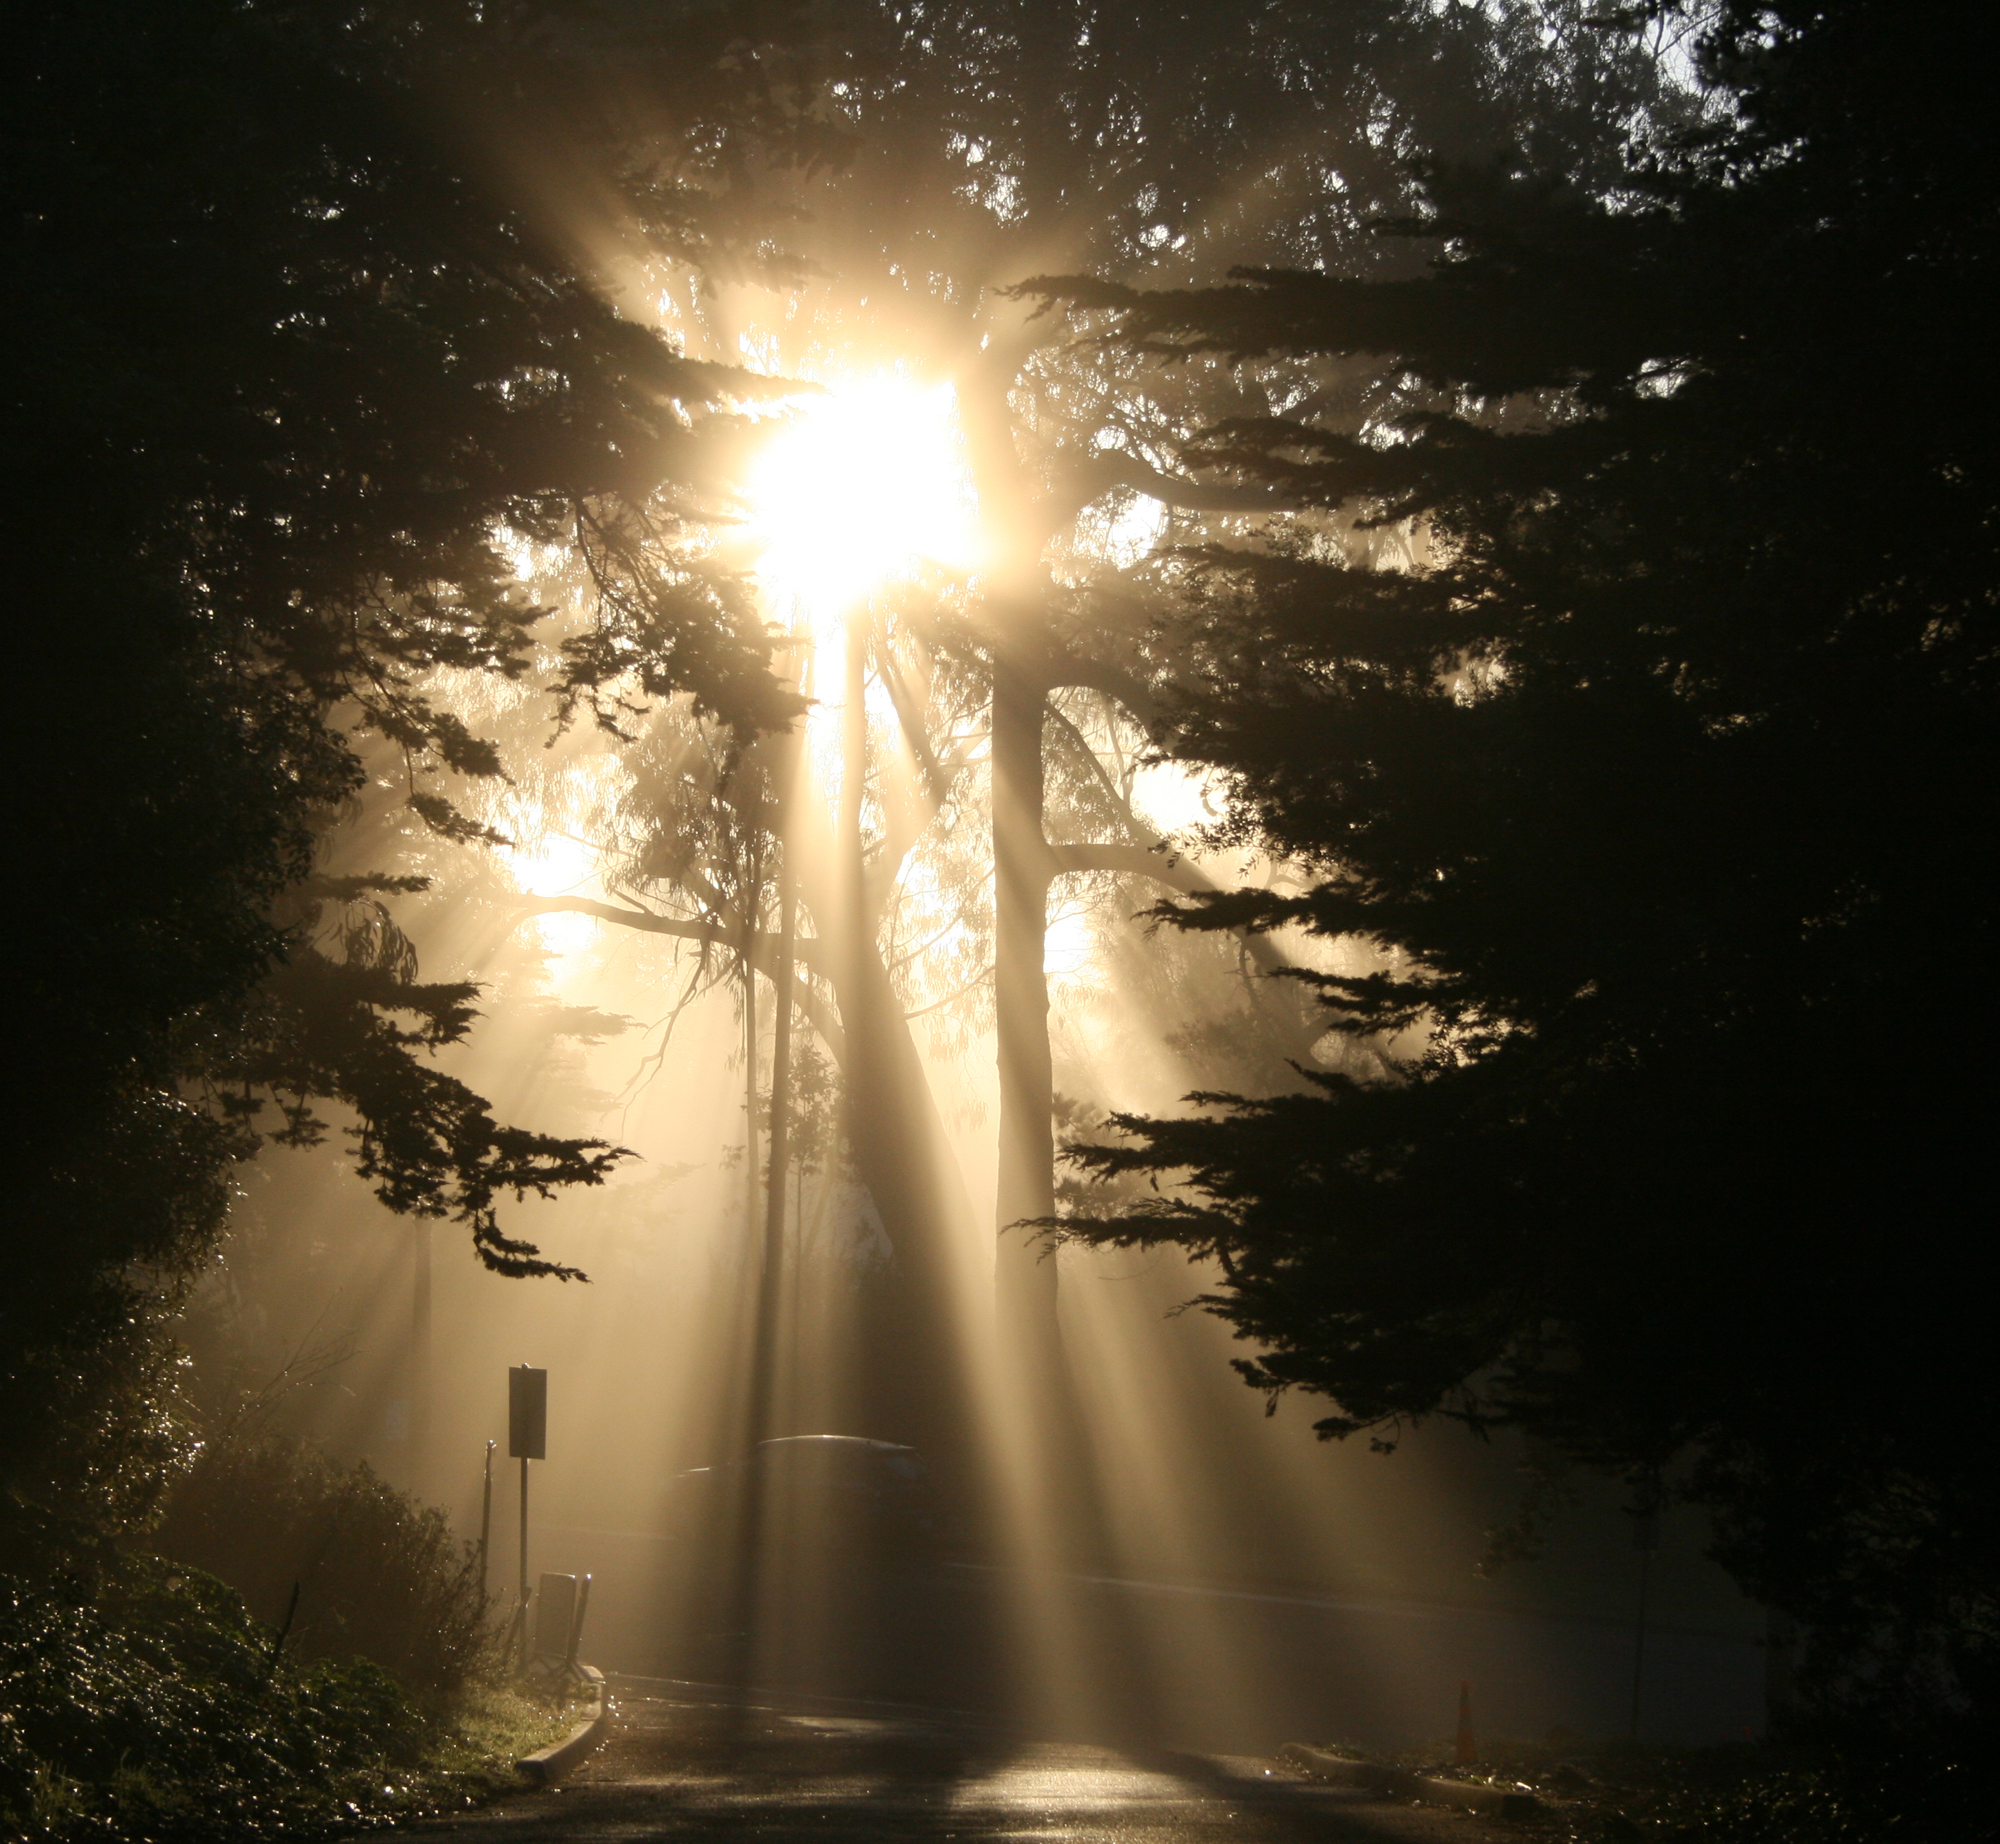
\includegraphics[height=250pt]{crep1}\end{center}
\section{Objective}
To achieve the above render, we make use of two well-known techniques namely Ray Tracing and Volumteric Shadowing. Ray Tracing is a technique for generating an image by tracing the path of light. Volumetric Shadowing is a technique that allows the viewer to see shadow beams called crepescular rays.
\newpage
\tableofcontents
\newpage
\fancyhf{}
\fancyhead[RE,LO]{Crepescular Rays}
\fancyhead[LE,RO]{Introduction}
\fancyfoot[CE,CO]{\leftmark}
\fancyfoot[LE,RO]{\thepage}
\renewcommand{\headrulewidth}{1pt}
\renewcommand{\footrulewidth}{1pt}
\section{Introduction}
The Ray Tracing algorithm very much mimics the procedure of observing the color of an object in nature. A light source emits a ray of light which travels, eventually, to a surface that interrupts its progress. One can think of this "ray" as a stream of photons traveling along the same path. There are two basic ideas for ray tracing.
\par
Forward ray tracing and backward ray-tracing. Forward ray-tracing is how the color of an object is observed by the eye in real life. That is, a ray of light is reflected of an object and travels into the eye producing an image. However, this algorithm is impractical because there will be many rays that will miss the camera and will not be useful to us. Thus, there will be a huge computational overhead. 
\par
For CG purposes, we make use of the backward ray-tracing algorithm. The basic idea is shoot a ray from the camera through each pixel of the image plane. If this ray intersects with an object, we send out another ray in the direction of our light source to determine if the object is under a shadow of another object. We also send out a reflected ray to obtain the reflection of another object if the object is capable of reflections.
\vspace{20pt}
\begin{figure}[h]
\centering
\fbox{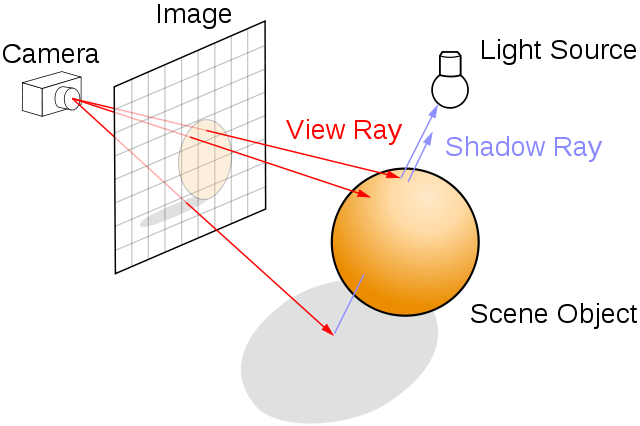
\includegraphics[width=0.8\textwidth]{ray_tracing_wiki}}
\caption{Basics of Ray Tracing}
\end{figure}
\newpage
The algorithm we have used to compute the volumetric rays is quite straightforward. We use the same concept used to compute shadows on the image plane. We start from the original image plane, compute shadows for every pixel on that image plane. Then we move the image plane towards the object and obtain a newer, smaller image plane. Compute shadows for this new image plane. This process is repeated until we reach the object.
The below image illustrates this process.
\vspace{20pt}
\begin{figure}[h]
\centering
\fbox{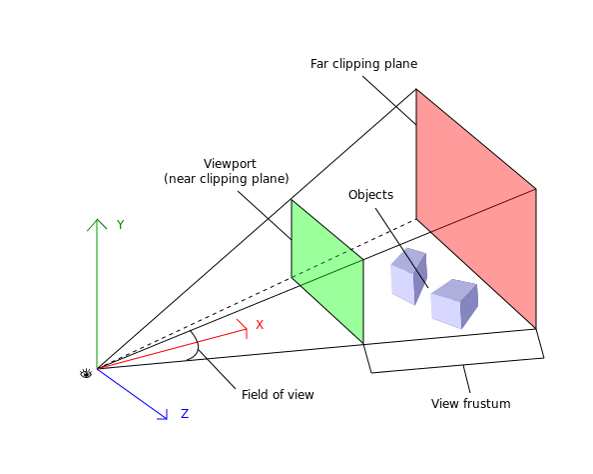
\includegraphics[width=0.8\textwidth]{volumetric_shadows}}
\caption{Basics of Volumetric Shadowing}
\end{figure}
\newpage
\section{System Schematic}
The System Schematic is a flowchart of operations done in different aspects of the project. Is represents the different modules in the program and thus depicts the flow of code.

\subsubsection{Ray Tracing}
\vspace{20pt}
\begin{figure}[h]
\centering
\fbox{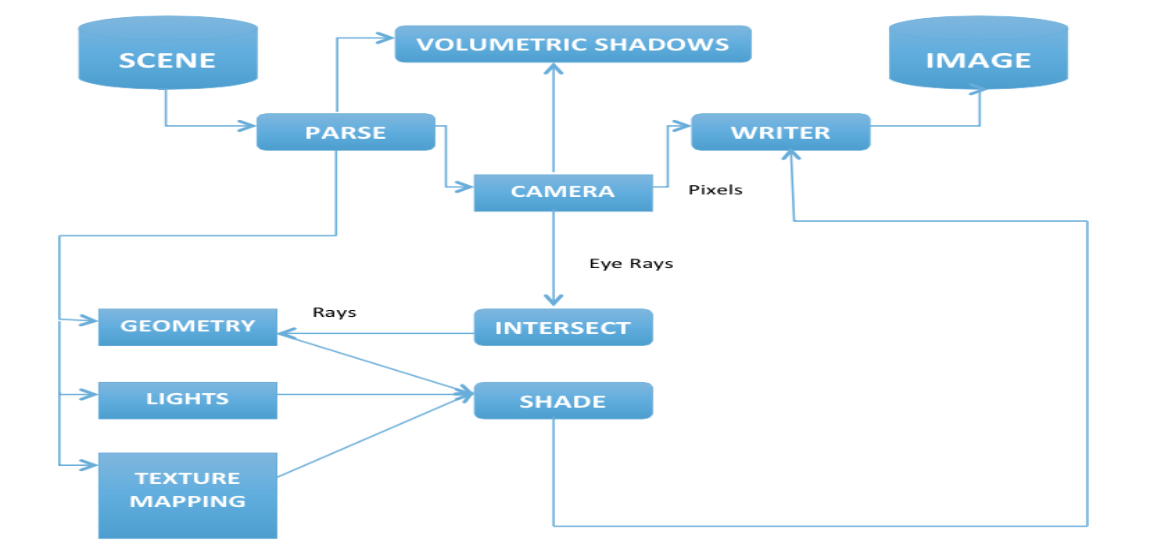
\includegraphics[width=0.8\textwidth, height=300pt]{RayTracingSchematic}}
\caption{System Schematic for Ray Tracing}
\end{figure}
\newpage
\subsubsection{Volumetric Shadowing}
\vspace{20pt}
\begin{figure}[h]
\centering
\fbox{\includegraphics[width=0.6\textwidth]{VolumetricShadows}}
\caption{System Schematic for Volumetric Shadowing}
\end{figure}


\subsubsection{Scan Line}
\vspace{20pt}
\begin{figure}[h]
\centering
\fbox{\includegraphics[width=0.8\textwidth]{ScanLine}}
\caption{System Schematic for Scan Line Rendering}
\end{figure}

\newpage
\section{Implementation}
\subsection{Scene Creation and Obj Format}
Since most objects out there use the v, vt, f and quadrilateral format, our program had to be modified to read data in that format and modify it into triangles.
\par
Moreover, a single leaf obj wouldn't suffice for the purposes of this project. So we took the same leaf obj, translated it, rotated it and scaled it to create a scene that represented falling leaves. All these combinations of leaves in different orientations were merged to create a single render. The scenes rendered can be dynamic or static.

\subsection{Backward Ray Tracing}
%%%\item Compute the Viewing Rays
\subsubsection{Compute the Camera Rays}
We represent a ray by obtaining the ray's origin and its direction. The first ray we look at is the viewing or camera ray. This ray is computed by making use of the camera position and the current pixel which has to be coloured. We first transform the pixel coordinates to $x, y \in [-1, 1]$.
\[ i = \dfrac{x * 2}{imagePlaneWidth} - 1 \]
\[ j = \dfrac{y * 2}{imagePlaneHeight} - 1 \]

The ray to the object can be represented by using the origin of the ray and the direction of the ray computed by using the object.
\[c_{n} = camera_{lookat}(c_{l}) + camera_{position}(c_{p}) \]
\[\overrightarrow{c_{v}} = camera_{lookat}(c_{l}) \times camera_{worldup}(c_{u}) \]
\[\hat{c_{v}} = \dfrac{\overrightarrow{c_{v}}}{\lvert \overrightarrow{c_{v}} \rvert} \]
\[ray\_camera\_to\_object_{position} (r_{p}) = c_{n} - c_{v} \cdot i - c_{u} \cdot j\]
\[ray\_camera\_to\_object_{direction} (\overrightarrow{r_{c}}) = r_{p} - c_{p} \]

\subsubsection{Compute the intersection of the camera ray\\ with the plane of the triangle}
Since there is no way knowing which triangle the ray will intersect with, we have to try out all triangles.
To check if the ray intersects with the plane of the triangle is easy. By finding out the normal to the triangle and taking the dot product of the ray and this normal we can verify if the triangle is parallel to the ray or starts behind the triangle or neither of those. 
\par
To begin with we need to make sure that we get the normal outwards rather than inwards. This will ensure that we get the correct normals. We first arrange all vertices in a counter-clockwise manner. If $v_{0}, v_{1} and v_{2}$ are the vertices in counter-clockwise order, then the normal is obtained by,
\[{n} = \overrightarrow{(v_{1}-v_{0})} \times \overrightarrow{(v_{2}-v_{0})}\]
\[\bigtriangleup _{normal} = \hat{n} = \dfrac{n}{\lvert n \rvert}\]

Then the dot product of the $\bigtriangleup _{normal}$ and the ray can provide us with information whether the $\bigtriangleup$ is parallel to the ray or not.
\[ \bigtriangleup _{normal} \cdot \overrightarrow{r_{c}}\ = 0 \implies \bigtriangleup \parallel \overrightarrow{r_{c}}\]

We are interested in the last condition because this signifies that the camera ray intersects the plane of the $\bigtriangleup$.

\subsubsection{Check if intersection point is inside the Triangle}
To obtain the point of intersection we must first compute the triangle distance:
\[d(\bigtriangleup) = \bigtriangleup_{normal} \cdot v_{0}\]
Then, the following equation gives us the distance to the plane:
\[d(plane) = -1 \times \dfrac{\bigtriangleup_{normal} \cdot (\overrightarrow{r_{c}} + (\bigtriangleup_{normal} \times -d(\bigtriangleup)))}{\bigtriangleup_{normal}\cdot \overrightarrow{r_{c}}}  \]
\[d(plane) < 0 \implies \bigtriangleup is\ behind\ the\ camera \]
Next we need to find the point that intersects with the plane.
This point, say $q$, is found by:
\[q = d(plane)\cdot\overrightarrow{r_{c}} + r_{p}\]
Now, that we have the point, we need to verify if this point lies inside the $\bigtriangleup$.
\[\dfrac{Area(q, v_{1}, v_{2}) + Area(q, v_{0}, v_{2}) + Area(q, v_{0}, v_{1})}{Area(v_{0}, v_{1}, v_{2})} \approx 1\]
If the above condition holds then our point is inside the $\bigtriangleup$.
\newpage
\subsection{Shadows}
From the point of intersection we need to shoot another ray in the direction of the light and find if it intersects with any of the objects. If it does, then that point is in shadow. But for the purposes of this project where the shadow falls on the image plane, we shoot out a ray from each pixel on the image plane in the direction of the light source (multiple shadows can be cast by shooting rays in the directions of the multiple light sources). This is done by performing the following calculations.
\[ s = \overrightarrow{l} + \overrightarrow{c_{l}} \]
\[ v = \overrightarrow{c_{u}} \times -\overrightarrow{c_{l}}\]

Transform the coordinates such that $x, y \in [-1, 1]$

\[ r_{l} = s - ((v \cdot -i) - (c_{l} \cdot -j) \]
\[ \overrightarrow{r_{l}} = \overrightarrow{l} - r_{l} \]
\[ \hat{r_{l}} = \dfrac{\overrightarrow{r_{l}}}{\lvert r_{l} \rvert} \]

Now that the light ray is calculated, we can go ahead and calculate the shadows by performing similar calculations done with the camera ray above, i.e. calculating the intersections and checking if it is contained in the triangle. If it is then the point is in shadow.
\par
The shadow rendered for a small leaf object.
\vspace{20pt}
\begin{figure}[h]
\centering
\fbox{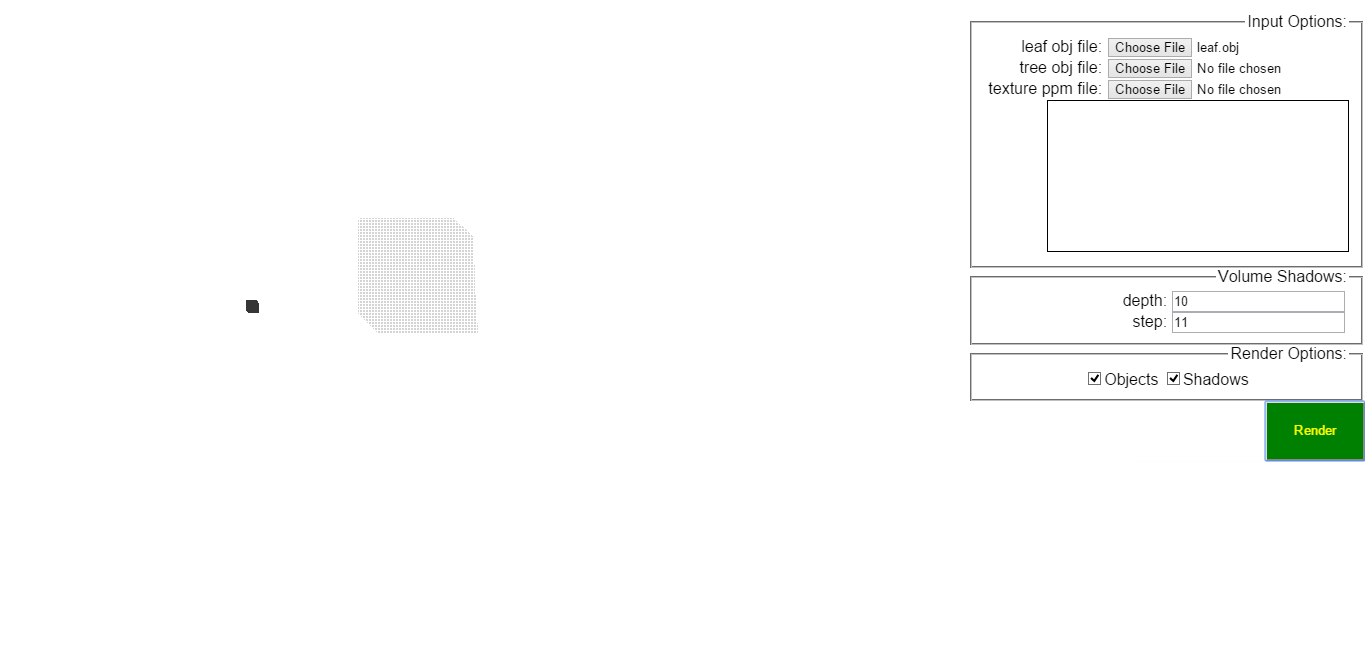
\includegraphics[width=0.6\textwidth]{single_leaf_single_shadow}}
\caption{Shadow for a single leaf using ray tracing}
\end{figure}

\newpage
\subsection{Volumetric Shadows}
The computation for Volumetric Shadows is very similar to computing shadows in ray tracing. The only difference here is that we compute the shadows for every step in the image plane, indicating that the image step is moving towards the object.
The image step indicates how fine the shadows will be. A lower shadow step will make the shadows more granular.
The ray from each pixel of the image plane to the light source will have a different equation with each render step.\
\[ \overrightarrow{r_{l}} = \overrightarrow{r_{l}} \cdot shadow\_step \]
\par The volumetric shadow rendered for a small leaf object.
\vspace{20pt}
\begin{figure}[h]
\centering
\fbox{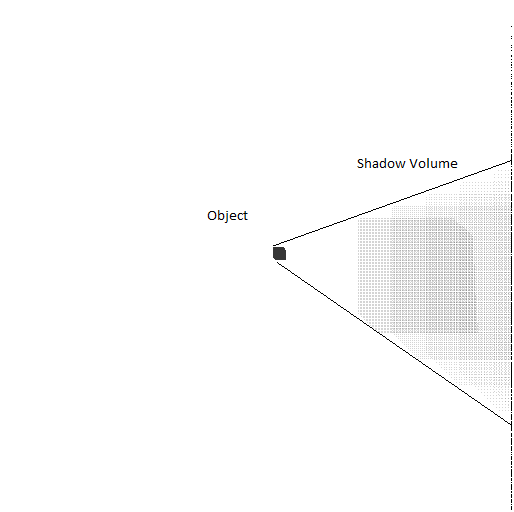
\includegraphics[width=0.8\textwidth]{single_leaf_shadow_volume_for_ppt}}
\caption{Volumetric Shadow for a single leaf with a large step size}
\end{figure}

\newpage
\section{Results}

\vspace{20pt}
\begin{figure}[h]
\centering
\begin{subfigure}{0.5\textwidth}
\centering
\fbox{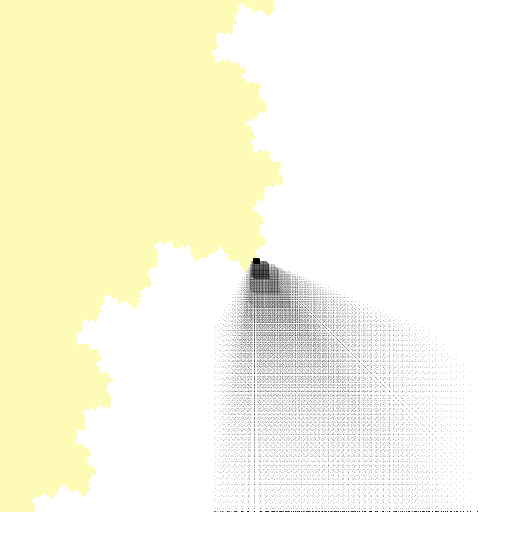
\includegraphics[width=0.7\textwidth]{object_and_volume_shadow_correct}}
\caption{A sun fractal acting as light source with a leaf producing volumetric shadows  (Took 28 min)}
\end{subfigure}%
\begin{subfigure}{0.5\textwidth}
\centering
\fbox{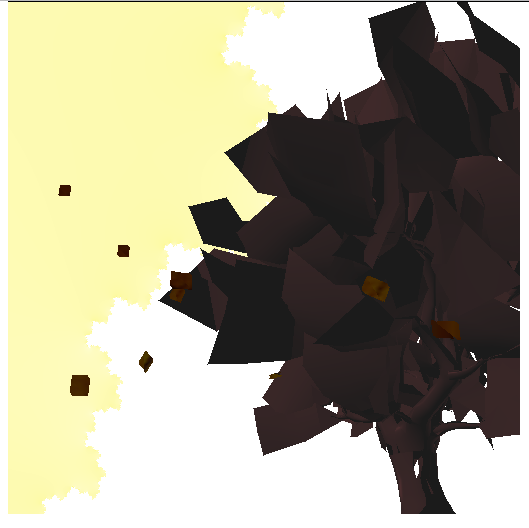
\includegraphics[width=0.7\textwidth]{scene_with_sun_fractal}}
\caption{Scene with a sun fractal, trees and leaves}
\end{subfigure}
\caption{Render of different scenes with a sun fractal}
\end{figure}

\vspace{20pt}
\begin{figure}[h]
\centering
\fbox{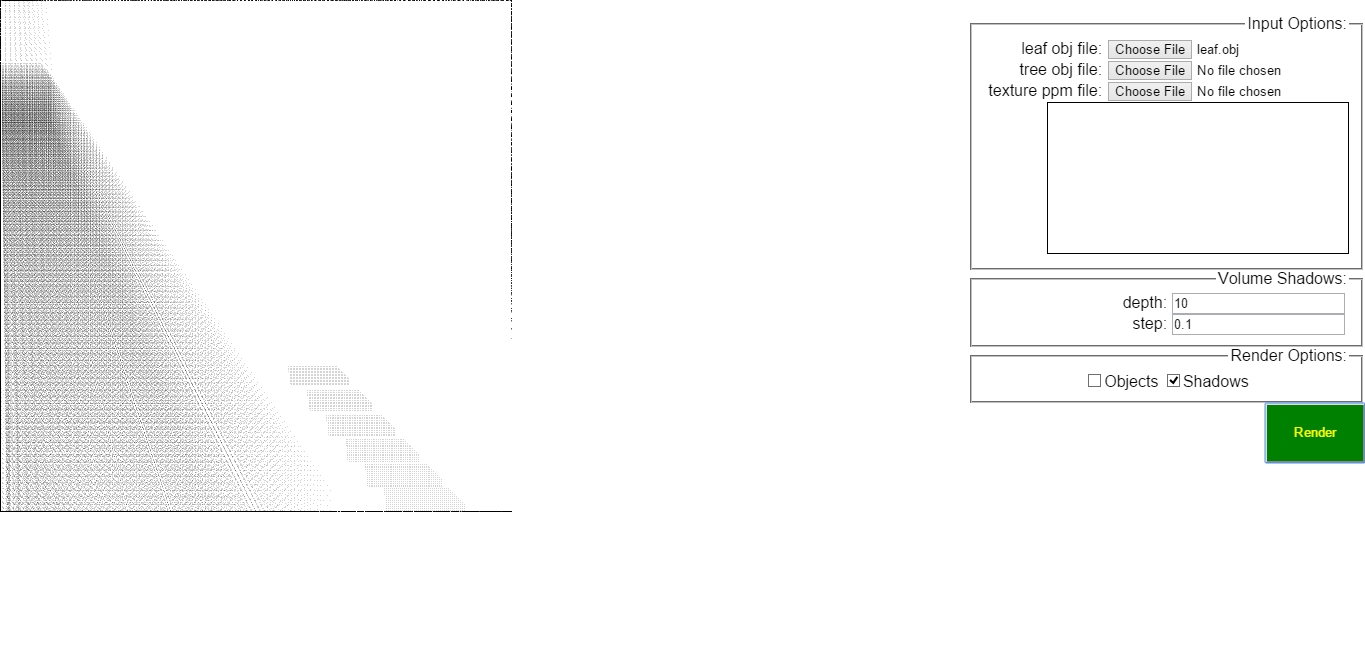
\includegraphics[width=0.8\textwidth]{multileaf_shadowVolume}}
\caption{Render of multiple leaves with increased step size (Took 28 min)}
\end{figure}

\newpage
\section{Challenges}
\begin{itemize}
\item One of the biggest challenges in the project is the slow computation time of ray tracing. Since every pixel is rendered against every triangle in the scene. The computation time is very huge. Therefore the debugging is a longer and tiring process.
\item Visualizing everything in object space was a difficult process.
\item Using the correct light positions to get a shadow.
\item Volumteric Shadows were also very challenging. It was a fairly new algorithm.
\item The volumetric shadow calculation with a new ray at every intermediate plane led to a lot of calculations.
\end{itemize}
\section{Conclusion}
\par Although we did not arrive at the exact result we were hoping to, we have acheived the purpose of this project, that is to have a better understanding of ray tracing and volumetric shadowing techniques.
\par While researching and implementing Ray-Tracing we were exposed to many methods that showed us how to implement photorealistic images. We were also made aware of the enormous computations required in the ray-tracing algorithm. In the process, we also mastered the ray-tracing algorithm and found out various alternatives to perform certain tasks in ray-tracing.
\par We also investigated into the several ways volumetric shading is done. And since, the shadows fall on the camera, we tweaked the algorithm to produce desired result.

\nocite{*}
\printbibliography
%%% End document
\end{document}